\section{Recovering a probability law from continuous probes}
\label{sec:laws}

Suppose an experiment gives the expectation of any rational polygonal test
function on $[0,1]$ to a requested accuracy. Can it produce the finite laws and
couplings required by the repository's expectation packet? Reading the mass
of each half-open mesh cell would require a discontinuous test. We give a
reconstruction using continuous ramps. It admits arbitrary atoms, including
atoms at the endpoints and mesh vertices.

\subsection{A finite distance with attaining certificates on both sides}

A finite law is a sorted list of rational sites in $[0,1]$, with nonnegative rational
weights adding to one. Combine equal sites and discard zero weights if desired.
On the union of the supports of two laws insert $0$ and $1$, sort and write the
distinct sites as $z_0<\cdots<z_m$. Pad missing weights with zeros. Define
\[
 w_i=z_{i+1}-z_i,\quad d_i=p_i-q_i,\quad D_i=\sum_{j=0}^{i}d_j,
 \qquad W(p,q)=\sum_{i<m} w_i |D_i| .
\]
Inserting a vertex with zero weights splits one edge with unchanged discrepancy;
therefore the result is independent of the common grid. Symmetry and the
triangle inequality follow by taking the union of all grids and using the
rational absolute-value laws. A zero sum forces $D_i=0$ on each positive-width
edge and hence equality of the weights (the last by total mass).

\begin{lemma}[Finite transport and its dual]\label{lem:dual}
$W(p,q)$ is both the least rational coupling cost for the distance $|x-y|$ and
the largest value of $\sum_i d_i f(z_i)$ among rational polygonal functions $f$
of Lipschitz constant at most one. Both optimizers have explicit PR producers.
\end{lemma}
\begin{proof}
Write $P_i=\sum_{j\le i}p_j$, $Q_i=\sum_{j\le i}q_j$, and $P_{-1}=Q_{-1}=0$.
In a common mass coordinate $u\in[0,1)$, give site $z_i$ the interval
$[P_{i-1},P_i)$ for the first law and $[Q_{i-1},Q_i)$ for the second.
Use the rational lengths of pairwise intersections as coupling entries.
Each interval partitions against the other family's intervals, proving the
marginals. Across the edge $(z_i,z_{i+1})$, this coupling carries exactly
$|P_i-Q_i|$ units because the left-hand initial intervals in $u$ are nested.
Every other coupling has rightward minus leftward flow $P_i-Q_i$ there,
and hence gross flow at least $|P_i-Q_i|$. The distance between any two
sites is the sum of the widths of the edges crossed. Summing first by edges
proves both the lower bound and attainment. Merging the sorted cumulative
endpoints emits at most $s+t-1$ nonempty overlaps for $s,t$ positive support
sizes. Advancing past a shared endpoint moves both cursors.

Discrete summation by parts gives
\[
 \sum_{i=0}^m d_i f(z_i)
 =\sum_{i<m}D_i\big(f(z_i)-f(z_{i+1})\big);
\]
the missing boundary term is $D_m f(z_m)=0$. Every 1-Lipschitz test bounds
the absolute value by $W$. Start with $f(z_0)=0$ and give the test a drop of
$w_i$ when $D_i\ge0$, and a drop of $-w_i$ otherwise. Linear interpolation
gives a rational 1-Lipschitz test attaining $W$. All sign decisions concern
finite rational discrepancies.
\end{proof}

This is the finite version of the one-dimensional Wasserstein identity of
Vallander. It gives a certificate of optimality checkable by a scan of the
sorted lists. Sorting unordered inputs is an extra cost. On an already sorted
common grid, cost, potential and sparse coupling each require only a linear
number of rational comparisons and arithmetic operations. A dense coupling
matrix could have $st$ entries. These operation counts do not bound the cost
of arithmetic on numerators and denominators.

\subsection{Two presentations and their finite contracts}

Let $\PL$ consist of continuous piecewise-linear functions with rational nodes
and ordinates on $[0,1]$. Equal polygonal functions can have different node lists.
Unions of node grids decide equality, positivity, and uniform rational bounds,
and compute the Lipschitz constant as the largest absolute slope.
\begin{itemize}
\item An \emph{expectation presentation} is an evaluator $A(f,r)$ with absolute
error $e_r$ for a scalar name $L(f)$, extensional in the polygon. Its contracts
are $L(1)=1$, rational linearity, and positivity $0\le f\Rightarrow 0\le L(f)$.
Rational linearity may be supplied as
$L(g+cf)=L(g)+cL(f)$ for rational $c$. For a numerical version,
$|A(g+cf,r)-A(g,s)-cA(f,t)|\le e_r+e_s+|c|e_t$.
Supply regularity, the analogous normalization and positivity contracts, and
extensionality under regridding. These all quantify over natural codes.
\item A \emph{law presentation} produces a finite rational law $M_p$ for each
$p$ with $W(M_p,M_q)\le e_p+e_q$. Its equivalence relation compares the two
different families by the same cross-bound. Lemma~\ref{lem:dual} supplies a
pairwise coupling and a distinguishing test at any two levels. Shifting both
indices by one gives the one-sided bound $W(M_{p+1},M_{q+1})\le e_p$ for
$q\ge p$ used in the repository packet.
\end{itemize}
Positivity and normalization imply $|L(f)-L(g)|\le b$ whenever
$\|f-g\|_\infty\le b$ for rational $b$. Apply positivity to each of
$b\mathbf 1\pm(f-g)$. This proof handles negative test values and also proves
monotonicity. A fixed PR realization of either presentation gives an iPRA
schema. An arbitrary external oracle gives the corresponding Type-2
construction.

\subsection{Reconstruction with a precision bound independent of the number of bins}

Let $N=2^n$, $h=1/N$, $x_i=ih$. For $0\le i<N$ let $B_i$ be the
polygon which is $1$ up to $x_i$, drops linearly to zero on
$[x_i,x_{i+1}]$, and is zero thereafter. This definition includes $i=0$
and $i=N-1$. The cumulative probes $C_i=L(B_i)$ are nondecreasing in $i$
and lie in $[0,1]$. Their differences are named scalars; the algorithm
never has to determine the sign of a named scalar. Read $a_i=A(B_i,r)$,
clip each rational reading to $[0,1]$, and set
\[
 b_{-1}=0,\qquad b_i=\max\{b_{i-1},\min(1,\max(0,a_i))\},\qquad b_N=1.
\]
Put mass $b_i-b_{i-1}$ at $x_i$ for $0\le i\le N$ and call the resulting
finite rational law $M(n,r)$. Nonnegative masses sum to one. For every
$i<N$,
\begin{equation}
                         |b_i-C_i|\le e_r.                 \label{eq:repair}
\end{equation}
Indeed clipping preserves the interval error about $C_j\in[0,1]$. The latest
reading gives the lower bound. Each previous clipped reading is at most
$C_j+e_r\le C_i+e_r$, so their maximum satisfies the same upper bound. The
repair has no factor of $N$ in its precision budget.

\begin{theorem}[Polygonal expectations and transport names]\label{thm:law}
For a rational polygon $f$ of Lipschitz constant $K$,
\[
 \big| L(f)-M(n,r)(f)\big|\le K\bigl(2^{-n-1}+2^{-r}\bigr),
 \qquad M(f):=\sum_i M_i f(x_i).
\]
Taking $n=r=p+2$ produces a law name from an expectation presentation. Conversely,
a law name gives an expectation presentation. Both round trips preserve
all observations up to equality of names.
\end{theorem}
\begin{proof}
Let $I_h f$ interpolate $f(x_i)$ on the mesh. At $x=x_i+th$, $0\le t\le1$,
the interpolation error is bounded by
$(1-t)Kth+tK(1-t)h\le Kh/2$. For rational polygons these inequalities need
only be tested at the union of the breakpoints. On each mesh cell the following
identity is verified by interpolation at its endpoints:
\[
 I_hf=f(x_N)\mathbf 1+
              \sum_{i<N}\big(f(x_i)-f(x_{i+1})\big)B_i.
\]
Taking $L$ and comparing to the identical telescoping formula for $M(n,r)(f)$
uses \eqref{eq:repair} with weights $|f(x_i)-f(x_{i+1})|$. Their sum is at
most $K\sum_i h=K$. The interpolation bound and the positive-functional norm
bound add the remaining $Kh/2$.

To compare two outputs at levels $p,q$, construct the maximizing polygon for
those exact rational outputs by Lemma~\ref{lem:dual}. Its Lipschitz constant
is one. Applying the displayed approximation twice against the same $L$
bounds $W$ by $3(e_p+e_q)/8$. The same argument works for equivalent
functional presentations because their agreement on every rational polygon applies to this particular test. This is
the two-run rule of Section~\ref{sec:basis} with a computable choice of a
separating observation.

In the reverse direction choose $j$ so that $K2^{-j}\le e_p$ and return
$M_j(f)$. For example take $j=p+\lceil\log_2(1+\lceil K\rceil)\rceil$;
the integer logarithm is a bounded search. The zero function and constant
polygons need no special branch. Lemma~\ref{lem:dual}, or its coupling proof
applied to a $K$-Lipschitz test, bounds two answers by $K(e_j+e_l)$.
This defines $L_M(f)$. To prove linearity evaluate all terms on the
same sufficiently fine law. Finite expectations are exactly rational-linear,
and the error of replacing each level is bounded by its own slope times
the two scale errors. Eliminating the common auxiliary level proves named
linearity. Positivity, normalization and regridding follow directly.

Starting at $L$, the first estimate shows that the resulting evaluator has
the same scalar value on each $f$. Starting at a law name $M$, let $P_p$
be the law reconstructed from $L_M$. Given $p,q$ synthesize the maximizing
polygon for $(P_p,M_q)$. Its expectations in $P_p$ and $M_q$ differ from
$L_M(f)$ by at most $3e_p/8$ and $e_q$ respectively, the second inequality
following by sending an auxiliary stage to arbitrary precision. Hence
$W(P_p,M_q)\le e_p+e_q$. This proves both round trips.
\end{proof}

A ramp has at most four vertices even when $N$ is large. Producing the full
grid law uses $N$ oracle answers at absolute error $2^{-r}$, $N$ prefix updates,
and $N+1$ output slots. Estimating $N$ individual bins with unrelated errors
and bounding their sum by $N$ times the worst error would cost up to $n$
additional guard bits. The cumulative probes avoid that loss in the
\emph{absolute-error oracle for arbitrary polygons} specified above. If the
interface accepts only unit-Lipschitz tests, $B_i$ has slope magnitude $N$ and
one calls the oracle on $B_i/N$ at precision $r+n$ before rescaling. The
cost claim depends on this distinction. Normalized dyadic answers of prescribed
precision are available by one guard bit and rational rounding if the basic
evaluator returns arbitrary fractions.

\paragraph{A law with atoms and deliberately inconsistent readings.}
Take density $1/4$ on $[0,1]$ and atoms of mass $1/7,1/4,5/14$ at
$0,3/7,1$ respectively. At every even probe add $2^{-r}$ to the exact answer;
at every odd probe subtract it. With $n=r=4$ the repair raises seven readings.
The exact transport distance to the original law is $2935/50176$, within
the certified $3/32$. The independent calculation in
\texttt{examples/laws.py} integrates the absolute CDF difference on each
affine segment, splitting at its zero if the sign changes.
\begin{center}
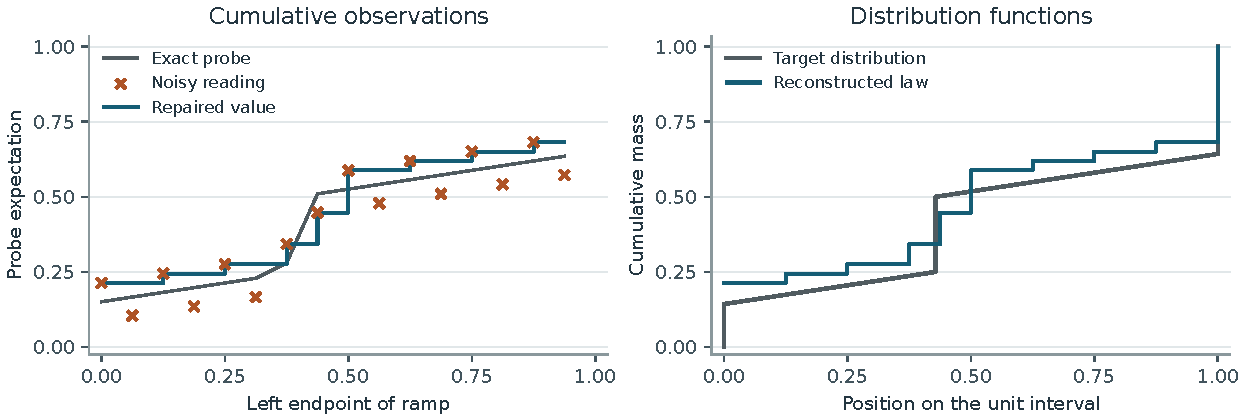
\includegraphics[width=.98\linewidth]{figures/ramp-repair.pdf}
\end{center}
The repair operates on cumulative ramp expectations. Their successive
differences define the atoms of the reconstructed law. The target's jumps at
$0,3/7,1$ are all admitted by the reconstruction theorem.

\subsection{Making the induction first-order}

The expression $\sum_i d_i L(B_i)$ in the proof abbreviates a finite
calculation. Here is a direct expansion which avoids induction on a statement
about arbitrarily many named scalars. Write $d_i=f(x_i)-f(x_{i+1})$ and
$S_0=f(x_N)\mathbf 1$, $S_{j+1}=S_j+d_j B_j$. Fix $r,t,n,f$ before
induction. The input's affine contract gives the rational inequality
\[
 |A(S_{j+1},t)-A(S_j,t)-d_jA(B_j,t)|\le(2+|d_j|)e_t.
\]
Telescope with induction on the cleared signed numerators, starting from
$|A(S_0,t)-f(x_N)|\le e_t$ by normalization and rational linearity with
auxiliary slack eliminated. The discrepancy between $A(S_N,t)$ and
$f(x_N)+\sum_{i<N}d_i A(B_i,t)$ is at most $(1+2N+K)e_t$.
For the prefix claim fix target index $i$ and use the upper bound
$A(B_i,t)+e_t+e_r$ for each of the first $i+1$ clipped samples.
Monotonicity of the true probes gives this finite bound by the rational
slack rule. The latest sample gives the converse lower bound with the same
slack. Both conclusions are inequalities between rationals. Letting the
auxiliary $t$ have enough bits for the final comparison recovers the displayed
constants. The proof can use finer readings than the law producer; those
readings do not enter its query budget.

\texttt{lean/PrefixObject.lean} defines the prefix accumulator as an actual
binary PR symbol parameterized by the syntactic body of a sample. It proves
inside the object calculus that the accumulator increases, covers the current
sample, and is bounded at a variable length $N$ by any common upper bound for
the first $N$ samples. Its induction matrix is
$i\le N\Rightarrow\mathrm{prefix}(i,x)\le u$. To use an integer upper bound,
multiply the finitely many positive denominators, including that of $u$, and
scale the clipped samples before applying the lemma. When a proposed upper
bound is negative the premises with any nonnegative sample give a finite
contradiction; empty prefixes have bound zero whenever $u\ge0$.
The signed Abel identity and construction of an attaining test are checked
in ambient Lean in \texttt{lean/LineDual.lean}.

\subsection{What becomes computable, and what still needs information}

\paragraph{Beyond Lipschitz tests.}
A rational-point evaluator for a continuous $g$ with a supplied modulus
$\omega$ satisfying $|x-y|\le2^{-\omega(k)}\Rightarrow |g(x)-g(y)|\le e_k$
gives a polygonal surrogate. Use mesh $2^{-\omega(p+2)}$, read its nodal
values with error $e_{p+2}$, and interpolate. Convexity of interpolation
bounds the uniform error by $2e_{p+2}$. Evaluate the resulting polygon
under the law presentation to accuracy $e_{p+1}$. The sum is at most $e_p$.
To compare two such estimates, apply the functional norm bound to their
polygons on a common refined grid. Thus the functional extends constructively
to all functions with this presentation. A Borel probability on the usual
unit interval yields such a functional semantically; the arithmetic
construction uses only its numerical input. No assertion about all subsets of
the interval is needed.

\paragraph{A discontinuous question about the law.}
Fix rational $0<t<1$. The map taking a law to its mass in $[0,t]$ cannot
have a continuous realizer on all these names. The laws $\delta_t$ and
$\delta_{t+s}$ have $W=s$ and give answers $1$ and $0$ whenever
$0<s\le1-t$. More directly, run a proposed finite reader at precision two on
the constant name $\delta_t$. For any finite set of indices read, pick
positive rational $s$ smaller than their radii and $1-t$.
A name can agree on those observations and use $\delta_{t+s}$ everywhere
else; its regularity follows from $W=s$. The same output cannot be within
$1/4$ of both answers.

A positive replacement is available given a rational width $\eta(p)>0$ at
which the mass in $(t-\eta,t+\eta)$ is bounded by $e_{p+2}$, with a
checkable presentation of this premise. Use lower and upper rational ramps
$g^-,g^+$ that go from $1$ to $0$ on $[t-\eta,t]$ and $[t,t+\eta]$,
restricted to $[0,1]$. They bracket the indicator and their difference vanishes
outside the open interval. An entirely numerical version of the premise
is $0\le L(g^+-g^-)\le e_{p+2}$. Evaluate the two polygonal tests within
$e_{p+2}$ and enlarge the resulting endpoints by $e_{p+2}$. This encloses
the desired value in a rational interval of width at most $5e_{p+2}$;
its midpoint has error at most $5e_{p+2}/2<e_p$. Even without a background
measure these midpoints are coherent: every lower ramp is bounded by every
upper ramp, so any two certified intervals overlap. The coherence estimate
then follows by adding the two radii. This specifies exactly what extra
information recovers the discontinuous observable.

Finally, an optimal coupling certifies distance between \emph{laws}. If a
prior application needs two random variables on a specified joint space,
the marginals do not determine their dependence. Two fair bits can be equal
almost surely or opposite almost surely with the same marginals. The
construction above supplies one joint realization for transport and Lipschitz
expectations. It preserves an already prescribed joint law only when additional
compatibility evidence is given.
